% Options for packages loaded elsewhere
\PassOptionsToPackage{unicode}{hyperref}
\PassOptionsToPackage{hyphens}{url}
%
\documentclass[
]{article}
\usepackage{amsmath,amssymb}
\usepackage{lmodern}
\usepackage{iftex}
\ifPDFTeX
  \usepackage[T1]{fontenc}
  \usepackage[utf8]{inputenc}
  \usepackage{textcomp} % provide euro and other symbols
\else % if luatex or xetex
  \usepackage{unicode-math}
  \defaultfontfeatures{Scale=MatchLowercase}
  \defaultfontfeatures[\rmfamily]{Ligatures=TeX,Scale=1}
\fi
% Use upquote if available, for straight quotes in verbatim environments
\IfFileExists{upquote.sty}{\usepackage{upquote}}{}
\IfFileExists{microtype.sty}{% use microtype if available
  \usepackage[]{microtype}
  \UseMicrotypeSet[protrusion]{basicmath} % disable protrusion for tt fonts
}{}
\makeatletter
\@ifundefined{KOMAClassName}{% if non-KOMA class
  \IfFileExists{parskip.sty}{%
    \usepackage{parskip}
  }{% else
    \setlength{\parindent}{0pt}
    \setlength{\parskip}{6pt plus 2pt minus 1pt}}
}{% if KOMA class
  \KOMAoptions{parskip=half}}
\makeatother
\usepackage{xcolor}
\usepackage{longtable,booktabs,array}
\usepackage{calc} % for calculating minipage widths
% Correct order of tables after \paragraph or \subparagraph
\usepackage{etoolbox}
\makeatletter
\patchcmd\longtable{\par}{\if@noskipsec\mbox{}\fi\par}{}{}
\makeatother
% Allow footnotes in longtable head/foot
\IfFileExists{footnotehyper.sty}{\usepackage{footnotehyper}}{\usepackage{footnote}}
\makesavenoteenv{longtable}
\usepackage{graphicx}
\makeatletter
\def\maxwidth{\ifdim\Gin@nat@width>\linewidth\linewidth\else\Gin@nat@width\fi}
\def\maxheight{\ifdim\Gin@nat@height>\textheight\textheight\else\Gin@nat@height\fi}
\makeatother
% Scale images if necessary, so that they will not overflow the page
% margins by default, and it is still possible to overwrite the defaults
% using explicit options in \includegraphics[width, height, ...]{}
\setkeys{Gin}{width=\maxwidth,height=\maxheight,keepaspectratio}
% Set default figure placement to htbp
\makeatletter
\def\fps@figure{htbp}
\makeatother
\setlength{\emergencystretch}{3em} % prevent overfull lines
\providecommand{\tightlist}{%
  \setlength{\itemsep}{0pt}\setlength{\parskip}{0pt}}
\setcounter{secnumdepth}{5}
\usepackage{booktabs}

\usepackage{longtable}
\usepackage{array}
\usepackage{multirow}
\usepackage{wrapfig}
\usepackage{float}
\usepackage{colortbl}
\usepackage{pdflscape}
\usepackage{tabu}
\usepackage{threeparttable}
\usepackage{threeparttablex}
\usepackage[normalem]{ulem}
\usepackage[utf8]{inputenc}
\usepackage{makecell}
\usepackage{xcolor}
\usepackage{siunitx}
\usepackage{booktabs}
\usepackage{longtable}
\usepackage{array}
\usepackage{multirow}
\usepackage{wrapfig}
\usepackage{float}
\usepackage{colortbl}
\usepackage{pdflscape}
\usepackage{tabu}
\usepackage{threeparttable}
\usepackage{threeparttablex}
\usepackage[normalem]{ulem}
\usepackage{makecell}
\usepackage{xcolor}
\ifLuaTeX
  \usepackage{selnolig}  % disable illegal ligatures
\fi
\IfFileExists{bookmark.sty}{\usepackage{bookmark}}{\usepackage{hyperref}}
\IfFileExists{xurl.sty}{\usepackage{xurl}}{} % add URL line breaks if available
\urlstyle{same} % disable monospaced font for URLs
\hypersetup{
  pdftitle={Article Long Title},
  pdfkeywords={Accessibility, Passive Data, Location Choice},
  hidelinks,
  pdfcreator={LaTeX via pandoc}}

\title{Article Long Title}
\author{true \and true \and true}
\date{2022-09-19}

\begin{document}
\maketitle
\begin{abstract}
This is where the abstract should go.
\end{abstract}

{
\setcounter{tocdepth}{2}
\tableofcontents
}
\hypertarget{introduction}{%
\section{Introduction}\label{introduction}}

\hypertarget{problem-statement}{%
\subsection{Problem Statement}\label{problem-statement}}

In November of 2019, the Utah Transit Authority (UTA) began a partnership with VIA, a private mobility company. Under this partnership, UTA has supplemented its fixed-route services in south Salt Lake County with on-demand shuttles hailed through a mobile application. So-called ``microtransit'' offerings of this kind have the potential to efficiently extend UTA services into low-density areas and function as last-mile services for the regular fixed-route rail and bus network. UTA is interested in examining other areas where microtransit services can be effectively deployed.

\hypertarget{objectives}{%
\subsection{Objectives}\label{objectives}}

The primary objective of this research project is to identify possible geographic areas along the Wasatch Front where an on-demand microtransit system might most effectively operate. To do this, the research team will implement an on-demand microtransit system within a multi-agent simulation of daily activity patterns for the Wasatch Front Region. This simulation is presently under construction for other UDOT-sponsored research projects aimed at evaluating the potential effects of an on-demand transit system aimed at wheelchair users, and an additional USDOT-funded project to examine techniques to optimize microtransit services.

A secondary objective of this research will be to provide a template for UDOT and UTA to examine projects of this kind with a microsimulation model. Utah has invested a great deal of resources into fixed route, high-capacity transit lines such as UVX, TRAX, and FrontRunner. These services perform well and have relatively high ridership statistics, but many people not directly near the stations can have difficulty accessing them. UTA will use this research to identify other places on the Wasatch Front where microtransit offerings could be successful. UDOT could also use this methodology to study the potential effectiveness of such services in other areas, such as Logan, Moab, and Cedar City.

\hypertarget{scope}{%
\subsection{Scope}\label{scope}}

This analysis is being developed using BEAM: the modeling framework for Behavior, Energy, Autonomy, and Mobility developed by Lawrence Berkeley National Laboratory. This research takes the BEAM model as given, modifying only those parameters and implementations that are necessary to conduct the current analysis. For example, we will modify the BEAM code to enable geo-fenced microtransit operations, which are a critical component of the current research. We will not attempt to modify BEAM's multi-modal pathfinding algorithms, which may affect the current research but must be taken as given under the scope of this project.

\hypertarget{outline-of-report}{%
\subsection{Outline of Report}\label{outline-of-report}}

The report is organized into the following chapters:

\begin{enumerate}
\def\labelenumi{\arabic{enumi}.}
\tightlist
\item
  \textbf{Introduction:} This chapter.
\item
  \textbf{Literature Review:} An overview of previous efforts to understand microtransit systems and forecast their operations.
\item
  \textbf{Methodology:} Methods and data used to create the initial microsimulation scenario in the Salt Lake City region.
\item
  \textbf{Existing On-Demand Deployment:} Also, results of the simulation applied to the existing VIA deployment.
\item
  \textbf{Candidate Regions:} An evaluation of three additional regions selected by UTA and UDOT for simulation analysis.
\item
  \textbf{Recommendations and Conclusions}
\end{enumerate}

\hypertarget{literature-review}{%
\section{Literature Review}\label{literature-review}}

\hypertarget{overview}{%
\subsection{Overview}\label{overview}}

TODO: fix references

This chapter presents prior attempts in the academic and practical literature to understand, model, and predict ridership for on-demand transit systems. The literature highlights the power and flexibility of demand-based modeling. MATSim is an agent-based simulation that models individuals' behavior, and BEAM (an extension to MATSim) places even more focus on individuals. As our project deals with modeling the UTA on Demand by VIA pilot program in Salt Lake City, we additionally discuss the program and the results it has achieved so far. Ultimately, we conclude that we will be using BEAM to model this and other potential on-demand transit implementations.

\hypertarget{purposes-and-description-of-on-demand-transit}{%
\subsection{Purposes and Description of On-Demand Transit}\label{purposes-and-description-of-on-demand-transit}}

One aspect of traditional public transit is that the routes are usually fixed. It is not always feasible to extend these fixed-route systems into less densely populated areas (at least, not in a way that would reasonably service most of the residents) due to the high costs of capital and operation and the relatively low ridership that would result (Mineta Transportation Institute, 2012). However, public transit has many benefits such as reduced carbon emissions per person-mile and less traffic congestion (Buchanan, 2019; Gershon, 2005), and the lack of transit options in many suburban areas requires residents to overwhelmingly use personal vehicles as their main form of transportation (Gershon, 2005). This raises the question of the most effective and efficient way to increase transit ridership and decrease dependence on personal vehicles in these areas.

One possible solution is the introduction of microtransit services. Microtransit is a form of shared, on-demand transportation (ODT) in which passengers schedule rides and vehicle routing is updated in real time to efficiently transport its users. The vehicles used are usually a form of minibus that can hold several passengers at once (Shaheen et al., 2015). One key application of microtransit is for first- and last-mile transportation, connecting a wide area to the existing fixed-route network (Shaheen et al., 2015) and taking less time than walking or cycling. Decreasing this first/last mile travel time can increase job accessibility by allowing individuals to travel farther with the same travel time budget, and some microtransit services have been shown to decrease this time significantly (Kang \& Hamidi, 2019). Especially as smartphone ownership and usage continues to increase, microtransit is a promising option, as booking rides can be done within phone apps, making the user experience easier (Agatz et al., 2011).

\hypertarget{analysis-framework}{%
\subsubsection{Analysis framework}\label{analysis-framework}}

Alonso-González et al.~(2018) set out to create an analysis framework that can be used to evaluate ODT services, both in simulation and real-world application, in order to compare them to existing systems. The framework presented requires identifying several characteristics of the ODT system: coverage and routing, operating hours, vehicle characteristics, the booking system, and request acceptance criteria. Then several quantities are calculated or estimated, including generalized journey time and share of declined ODT trips as well as usage values. The ODT system is then compared with other modes such as fixed transit and walking/biking. The study concludes that a generalized cost of travel metric would be the most useful in comparing the ODT system against other options, as it was a good indicator of changes in mobility.

\hypertarget{previous-attempts-to-model-on-demand-transit}{%
\subsection{Previous Attempts to Model On-Demand Transit}\label{previous-attempts-to-model-on-demand-transit}}

Due to the high potential of ODT/microtransit services, many models and simulations have been created. Vosooghi et al.~(2017) published a literature review discussing several simulation software packages: Azevedo et al.~(2016) used SimMobility to model an autonomous taxi network, MobiTroop was used by Heilig et al.~(2015) to simulate carsharing in the Stuttgart, Germany area, and MATSim has been used to develop a carsharing model in Berlin (Ciari et al., 2014) and analyze one in Zurich (Balać et al., 2015), and it was used to model a shared autonomous vehicle system (Fagnant \& Kockelman, 2014).

Ronald et al.~(2017) looked at three software simulations in more detail: the basic simulation Delphi, the agent-based simulation MATSim, and the traffic microsimulation SUMOoD (SUMO on Demand). The study found that these simulations generally produced similar results with respect to number of vehicles and amount of demand, and noted that all simulations performed as expected based on real-world observations (Schofer et al., 2003). They are also quick to point out that results of these simulations might be optimistic if simplifications to routing are made or if using an undirected network, where a vehicle could pick up passengers on either side of a road no matter the direction of travel.

\hypertarget{matsim-and-beam}{%
\subsubsection{MATSim and BEAM}\label{matsim-and-beam}}

MATSim (short for ``Multi-Agent Transport Simulation'') is an open-source framework for transportation modeling originally developed in Zurich. The framework simulates traffic flows and congestion on a microscopic level, and simulates demand by creating agents and following their daily schedules and decisions. It is designed to model a single day in large-scale scenarios, and uses an iterative process to have each agent optimize their schedule and consider factors such as route choice, mode choice, time choice, and destination choice (Horni et al., 2016). This is similar to how many people would likely use a transportation network: either trying several options and sticking with what works best for them, or using a routing service (such as Google Maps) to find their optimal route. It is important to note that this is different than finding the optimal solution for the whole system (which likely would lead to some agents individually being assigned very poor routing/mode choice/etc.); each individual tries to optimize their own travel, and MATSim outputs the overall equilibrium that results (Horni et al., 2016). MATSim has been used in numerous studies to model various scenarios: Bischoff \& Maciejewski (2016) simulated a city-wide replacement of personal vehicles with autonomous taxis in Berlin, Cyganski et al.~(2018) introduced autonomous vehicles and ODT to Brunswick via simulation, and Viergutz \& Schmidt (2019) modeled ODT vs public transit in the rural town of Colditz.

BEAM, which stands for Behavior, Energy, Autonomy, and Mobility, is an extension to the MATSim framework, and is maintained by Lawrence Berkeley National Laboratory (BEAM - the Modeling Framework for Behavior, Energy, Autonomy, and Mobility, n.d.). The BEAM documentation (The BEAM Team, 2017) gives a description of some of its functions and purposes. The simulation is designed to simplify running full-scale transportation models, and places an emphasis on within-day agent mode choice and planning (as an example, after an agent requests a ODT vehicle, they may decide the wait time is too long and choose another mode). It is also intended to find the equilibrium point where resource markets (including road capacity and fleet availability) match the demand for service.

\hypertarget{real-world-microtransit}{%
\subsection{Real-World Microtransit}\label{real-world-microtransit}}

Microtransit/ODT has generally performed well in simulations; however, few ODT services have been implemented in the real world. Perhaps the most notable is Kutsuplus, which was implemented in Helsinki, Finland from 2102--2015. An official report of the system was created, but did not include an analysis regarding the mobility improvements compared with already-existing alternatives (Alonso-González et al., 2018; Kari, 2016).

\hypertarget{uta-on-demand-by-via}{%
\subsubsection{UTA On Demand by VIA}\label{uta-on-demand-by-via}}

Another real-world microtransit implementation began in November 2019, when Utah Transit Authority (UTA) partnered with VIA to run a pilot microtransit service, UTA on Demand, in southern Salt Lake County (Robertson et al., 2020). The two main goals of this program were to expand access to public transit, providing first- and last-mile connections, and increase mobility for all users, even on trips not involving fixed-route transit. The purpose of the pilot program was to determine if microtransit would achieve these goals effectively (Office of Communications \& Marketing, 2019).

As of the time of writing, monthly reports on the program are available from December 2019 through November 2020, as well as four quarterly reports. Several metrics were measured and compared to previously set goals in different areas, such as ridership, wait times, and cost per rider. At the end of the first quarter (December--February), the pilot program either met or was on track to meet the 6-month goals for each metric (Office of Communications \& Marketing, 2020a). However, due to the COVID-19 pandemic becoming prevalent in Utah beginning mid-March, significantly fewer people have utilized the service, and average ridership from March through November was significantly lower than the 6-month goals (Office of Communications \& Marketing, 2020c).

Though the pilot program did not meet the goals that were originally set, UTA renewed its contract with VIA for an additional year (Office of Communications \& Marketing, 2020c). This is in part because the program was projected to have met its 6-month goals in absence of the pandemic (Office of Communications \& Marketing, 2020b), and also more generally for continued evaluation and testing (Office of Communications \& Marketing, 2020c).

In September 2020, UTA released a report detailing a possible expansion of microtransit services to other areas in Utah following the UTA on Demand pilot program (Robertson et al., 2020). Three characteristics were considered: Transit potential, reflecting population and employment density; transit need, reflecting socio-economic factors that indicate a higher propensity to use transit; and the existing transit service level, based on quality and quantity of transit already available in the area. Based on these characteristics, 19 zones were identified between Brigham City and Santaquin as areas that could potentially benefit from microtransit services. Ridership was estimated based on number of residents and number of workers employed within each zone, as well as a mode share score that VIA developed based on their internal demand model. The report makes no definitive recommendation regarding expanding microtransit services, but does present several results of the analysis for each zone, including how well microtransit would improve transit coverage, provide efficient transit, replace existing bus routes, and increase equity. The report also notes several considerations regarding accessibility (including paratransit) and operations, and that this study will inform UTA's future transit choices.

\hypertarget{summary}{%
\subsection{Summary}\label{summary}}

Many different transportation simulation packages have been created and used in various situations. Part of this project involves developing a model that UTA can use for future research. Much of this work has been done previously in another UDOT-sponsored research project in developing a simulation including wheelchair-accessible microtransit vehicles. That project uses BEAM to develop its model, as BEAM effectively models individual user behavior in full-scale simulations. Because of this, we will be using BEAM as well in our research.

\hypertarget{methodology}{%
\section{Methodology}\label{methodology}}

\hypertarget{overview-1}{%
\subsection{Overview}\label{overview-1}}

This chapter describes the methodology we followed to generate the simulation scenarios. First, we will provide background information on BEAM itself, including the modifications to use geofencing for microtransit vehicles. This is followed by descriptions of the BEAM scenarios we developed for this research.

\hypertarget{beam}{%
\subsection{BEAM}\label{beam}}

Adaptive algorithm

Ride hailing versus transit

\hypertarget{geofencing-modifications}{%
\subsubsection{Geofencing Modifications}\label{geofencing-modifications}}

Adjusted ride hail matching algorithm to exclude requests from locations outside of a point.

\hypertarget{scenario-description}{%
\subsection{Scenario Description}\label{scenario-description}}

A BEAM scenario consists of the following:

\begin{itemize}
\tightlist
\item
  A description of transportation supply in the form of highway networks, transit services, and ride hail vehicles.
\item
  A description of travel demand, or the trips and activities for a synthetic population.
\item
  A configuration describing how the scenario operates and which modules are included.
\end{itemize}

\hypertarget{networks}{%
\subsubsection{Networks}\label{networks}}

Open

\hypertarget{demand}{%
\subsubsection{Demand}\label{demand}}

BEAM requires an input file representing trips and daily activities occurring in the region.

Synthetic population is developed in PopulationSim

Skims for transportation modes converted from WFRC / MAG model

ActivitySim

\hypertarget{configuration}{%
\subsubsection{Configuration}\label{configuration}}

\hypertarget{summary-1}{%
\subsection{Summary}\label{summary-1}}

Be smart about the figures and tables you include. Figures should be high resolution, and tables should always be table objects. If your table is an image of a table, I will place three pins in the voodoo dolls I keep for each of my RA's.

\hypertarget{existing-scenario-evaluation}{%
\section{Existing Scenario Evaluation}\label{existing-scenario-evaluation}}

\hypertarget{overview-2}{%
\subsection{Overview}\label{overview-2}}

UTA, in partnership with VIA, ran a pilot program of microtransit service in south Salt Lake County from November? 2019\textendash November? 2020. In order to assess the performance of our BEAM simulations when compared with real-world observed data, we compared the results of the two on several metrics:

\begin{verbatim}
## qs v0.25.4.
## ✔ skip target D
## ✔ skip target EX
## ✔ skip target B_fleet
## ✔ skip target UTAOD
## ✔ skip target A_fleet
## ✔ skip target C_fleet
## ✔ skip target D_fleet
## ✔ skip target EX_fleet
## ✔ skip target good_months
## ✔ skip target event_cols
## ✔ skip target A
## ✔ skip target B
## ✔ skip target C
## ✔ skip target fleets
## ✔ skip target UTA
## ✔ skip target scenarios
## ✔ skip target total_riders
## ✔ skip target average_wait_times
## ✔ skip target utilization
## ✔ skip target existing_comparison
## ✔ skip pipeline: 0.071 seconds
\end{verbatim}

\begin{table}
\centering
\begin{tabular}[t]{lrrr}
\toprule
  & Ridership & Utilization & Avg. wait time (min)\\
\midrule
UTA Observed Data & 347.3333 & 2.063333 & 11.33333\\
BEAM 'Existing' Scenario & 667.0000 & 1.317531 & 9.92500\\
\bottomrule
\end{tabular}
\end{table}

\hypertarget{summary-2}{%
\subsection{Summary}\label{summary-2}}

More Text

\hypertarget{candidate-region-evaluation}{%
\section{Candidate Region Evaluation}\label{candidate-region-evaluation}}

\hypertarget{overview-3}{%
\subsection{Overview}\label{overview-3}}

We created several scenarios with microtransit fleets in various areas. A map of these areas is given below:

\begin{figure}
\centering
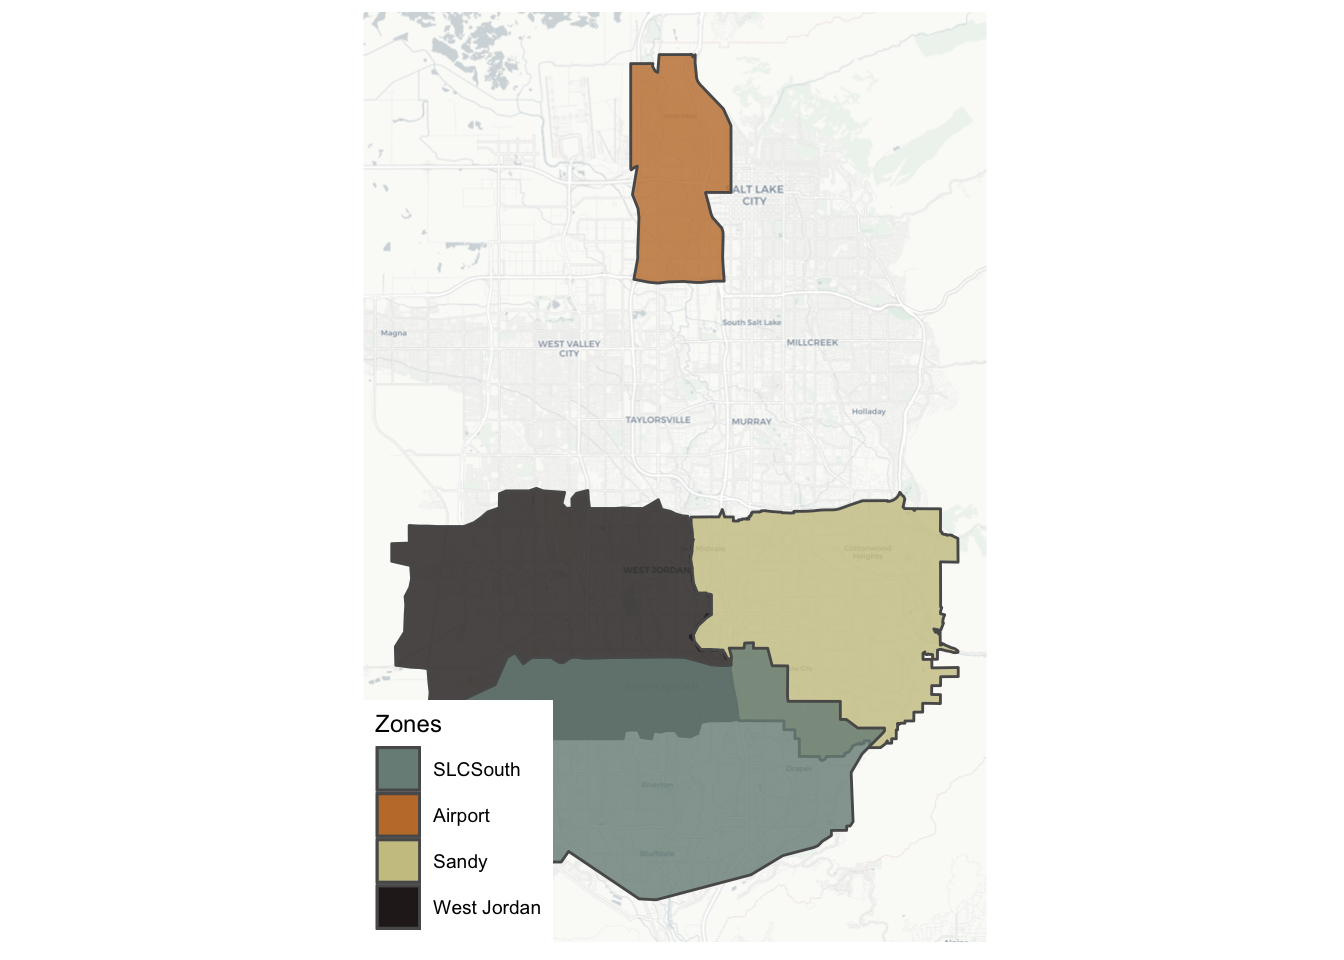
\includegraphics{microtransit_areas_files/figure-latex/map-1.pdf}
\caption{\label{fig:map}Ridehail zones in Salt Lake County.}
\end{figure}

The combinations of areas in each scenario is given:

TODO: add and reference that file here (it exists, just not in this repo yet)

And the results of our simulations:

\begin{verbatim}
## qs v0.25.4.
## ✔ skip target D
## ✔ skip target EX
## ✔ skip target B_fleet
## ✔ skip target UTAOD
## ✔ skip target A_fleet
## ✔ skip target C_fleet
## ✔ skip target D_fleet
## ✔ skip target EX_fleet
## ✔ skip target good_months
## ✔ skip target event_cols
## ✔ skip target A
## ✔ skip target B
## ✔ skip target C
## ✔ skip target fleets
## ✔ skip target UTA
## ✔ skip target scenarios
## ✔ skip target fleet_sizes
## ✔ skip target total_riders
## ✔ skip target average_wait_times
## ✔ skip target utilization
## ✔ skip target ridership_comparison
## ✔ skip target wait_time_comparison
## ✔ skip target utilization_comparison
## ✔ skip target existing_comparison
## ✔ skip target all_comparisons
## ✔ skip pipeline: 0.075 seconds
\end{verbatim}

\begin{verbatim}
## $`Existing comparison`
## # A tibble: 2 x 4
##   ` `                      Ridership Utilization `Avg. wait time (min)`
##   <chr>                        <dbl>       <dbl>                  <dbl>
## 1 UTA Observed Data             347.        2.06                  11.3 
## 2 BEAM 'Existing' Scenario      667         1.32                   9.93
## 
## $`Ridership comparison`
## # A tibble: 5 x 3
##   Scenario Entering Leaving
##   <chr>       <int>   <int>
## 1 existing      667     642
## 2 A             932     899
## 3 B             833     801
## 4 C            1079    1038
## 5 D            1571    1515
## 
## $`Utilization comparison`
## # A tibble: 5 x 3
##   Scenario Utilization `Fleet size`
##   <chr>          <dbl>        <int>
## 1 existing        1.32           25
## 2 A               1.39           33
## 3 B               1.29           32
## 4 C               1.30           41
## 5 D               1.39           56
## 
## $`Wait time comparison`
## # A tibble: 7 x 6
##   Quantile existing     A      B      C     D
##   <chr>       <dbl> <dbl>  <dbl>  <dbl> <dbl>
## 1 0%           1.13  0.95  0.867  0.783  0.55
## 2 10%          3.67  3.53  3.37   3.31   3.47
## 3 25%          5.77  5.68  5.7    5.57   5.54
## 4 50%          9.93  9.72 10.2    9.95   9.77
## 5 75%         13.5  13.4  13.4   13.3   13.1 
## 6 90%         15.5  15.5  15.5   15.6   15.4 
## 7 100%        19.2  21.1  18.3   18.9   18.3
\end{verbatim}

\hypertarget{summary-3}{%
\subsection{Summary}\label{summary-3}}

Other, more different text

\hypertarget{recommendations}{%
\section{Recommendations}\label{recommendations}}

\hypertarget{overview-4}{%
\subsection{Overview}\label{overview-4}}

Will we ever run out of text?

\hypertarget{summary-4}{%
\subsection{Summary}\label{summary-4}}

Of course not

\hypertarget{references}{%
\section*{References}\label{references}}
\addcontentsline{toc}{section}{References}

\end{document}
